\PassOptionsToPackage{no-math}{fontspec}
\documentclass[fontset=windows, 12pt]{article}
\usepackage[a4paper, total={6.5in, 10in}]{geometry}
\usepackage{ctex}
% \usepackage{xeCJK}
\usepackage{float}
\usepackage{graphicx}
\usepackage{amsmath}
\usepackage{bm}
\usepackage{mathspec}
% \usepackage{fontspec}
\usepackage{xcolor}
\usepackage{tcolorbox}
\usepackage{tikz}
\usepackage{tabularx}
\usepackage{framed}
\usepackage{booktabs}
%% 注意: 我注释了第65 行:mathspec.sty文件中引用fontspec宏包的命 
%% 到时候记得改回来, 已经加入了快速访问

\newcommand{\cmd}[2][\{*args\}]{\texttt{\textbackslash#2#1}}
\newcommand{\tb}[1]{\textbf{#1}}
\newcommand{\scale}[2]{
    \scalebox{#1}[#1]{#2}
}
\newcommand{\im}[1]{\ensuremath{\displaystyle #1}}

% 使用样例
% \scale{2}{A} this A is small than the

% Test scale Formulars:
% \scale{2}{\ensuremath{\sum}}
%
% \bigskip
% \scale{8}{\LaTeX}

%%  引用字体
% 这里定义一个test命令用于测试引用中文名称字体
% \newfontfamily{\test}{测试.ttf}



%% 设置全局的rm字体为Times New Roman 字体
% \setmainfont{Times New Roman}

% \newfontfeature{\testt}{MesloLGL Nerd Font}
% 注意:不能直接复制字体的名字,得进入字体属性中看正规得名字
%% 英文字体设置, 字体的属性(粗系斜)设置放在[]中,
% 不然你的组合命令: \bf{\comic Hello}中的hello无法加粗[斜体]
% 除此之外, 还可以设置字体的颜色这个可选参数:

\newfontfamily{\comic}{comic.ttf}[
    BoldFont=comicbd.ttf,
    ItalicFont=comici.ttf,
    BoldItalicFont=comicz.ttf
]

\newfontfamily{\comicblue}{comic.ttf}[Color=blue]
% 特殊字体的调用
\newfontfamily{\Meslo}{Meslo LG L Regular Nerd Font Complete.ttf}
\newfontfamily{\scp}[Path=../Fonts/]{SourceCodePro.otf}
% 注意:这个字体的调用有一个巨坑,下面的几个写法都是错误的
% \newfontfamily{\scp}[Path=../Fonts]{SourceCodeProTest.otf}
% \newfontfamily{\scp}{../Fonts/SourceCodeProTest.otf}
 

%% 中文字体设置
\newfontfamily{\Fangsong}{STFANGSO.TTF}
\newfontfamily{\Yahei}{msyh.ttc}

% 在上面我们都是设置的正文字体,如果要设置公式的字体就需要另外一个宏包: mathspec
% 注: 这个mathspec宏包和fontspec宏包其实是冲突的, 因为mathspec宏包会自动调用fontspec宏包

% 使用mathspec还有一个好处:就是可以设置包括数学公式字体的全部字体
% \setallmainfonts{Times New Roman}
% \setallmainfonts{STFANGSO.TTF}
% 注意:假如你把mathspec宏包中的65行应用fontpec的内容注释掉会报错:某些希腊符号已经被定义了
% 注意:设置中文的字体时,必须使用如下的选项:
% \setCJKmainfont{SIMYOU.ttf}
% 注意:这是部分的中文字体时,下面的和英文字体类似的命令是不起作用的
% \newfontfamily{\dengb}{SIMYOU.ttf}
\setCJKfamilyfont{dengb}{dengb.TTF}

% 可选参数是为了同时实现中英文伪粗体和伪斜体
\setCJKfamilyfont{yaoti}{FZSTK.TTF}[AutoFakeBold, AutoFakeSlant]

% 但是这个CJK命令仅仅只对中日韩文字有效果,想要设置英文字体和上面的类似
\newfontfamily{\yaoti}{FZSTK.TTF}

% 把同时设置中英文的命令进行一个封装
\newcommand{\Yaoti}{\yaoti \CJKfamily{yaoti}}


% 设置数学公式字体,注意:三个选项设置中间不能有空格
% \setmathfont(Digits, Greek, Latin){comic.ttf}
% \setmathfont(Digits,Greek,Latin)[
%     ItalicFont=comici.ttf,
%     BoldFont=comicbd.ttf,
%     BoldItalicFont=comicz.ttf
% ]{comic.ttf}
% 注意:如果没有给出新的数学字体的粗体和斜体的样式的话,LaTeX会给出警告





\title{字体调用}
\author{Eurake}
\date{} 
\begin{document}
\maketitle

\section{常见的字体格式}
我们常见的字体格式,无非就是这几种

\begin{framed}
    {\ttfamily .ttf~~.otf~~.ttc~~.ttc~~.woff~~.woff2~~.eot~~.pfb~~.afm~~.fon~~.pcf}
\end{framed}


下面我们梳理一下,从计算机读取文档,到生成最终的文字,到底中间都经历了一些什么。
\begin{framed}
\begin{enumerate}
    \item \textbf{编码【Encoding】:} 文字以字符串的形式存储在我们编写的文档中,
        使用字体的软件首先通过 \textbf{映射关系},找到各个字符对应的字形信息
    \item \textbf{定位:} 每一组信息分为两个部分,\textbf{度量信息}和 \textbf{图象信息(点阵或轮廓)}, 
        然后 \textbf{排版软件}安排每一个字符,行,段,把他 \textbf{定位}在一个二维平面上 \textbf{位置}
    \item \textbf{存储:} 我们常见的矢量图格式(PDF, EPS, SVG),主要就是存储这些元素的定位信息。
    \item \textbf{渲染:} 至于字符的图像信息,主要是在渲染到屏幕上和打印时才绘制(曲线)和填充(颜色)的
\end{enumerate}
\end{framed}

字体的渲染需要诸多的 \textbf{规则},这里就不细说 ... 
比如 \textbf{连写, 排序,重排} $\cdots$

{
    \ttfamily
    我能吞下玻璃而不伤身体。
}

\subsection{警惕空格的产生}
\begin{framed}
% \fbox{
\parbox[l][4em][l]{0.5\linewidth}{
以下是源码:

{\ttfamily
Hel

lo%
}}
\parbox[l][4em][l]{0.45\linewidth}{
运行结果:
Hel
lo
}%}   
\end{framed}

\clearpage
\section{字体的调用}
\subsection{系统字体}
\begin{figure}[!htb]
    \begin{minipage}[c]{0.25\linewidth}
            \centering
            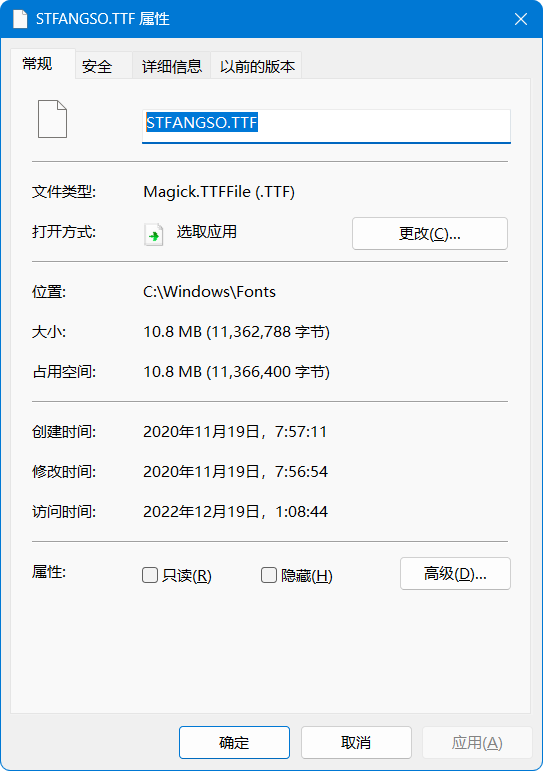
\includegraphics[scale=0.25]{../Pic/字体选择.png}
            \label{1}
            \caption{字体选择备注1}
    \end{minipage}
    \hfill
    \begin{minipage}[c]{0.6\linewidth}
        \centering
        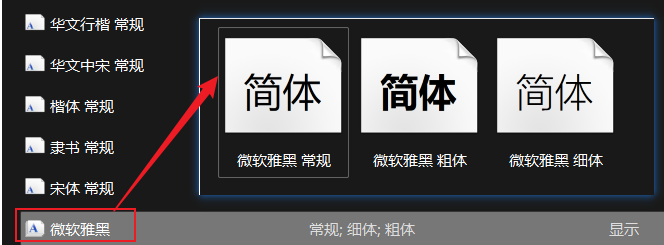
\includegraphics[scale=0.5]{../Pic/字体选择2.png}
        \label{2}
        \caption{字体选择备注2}
    \end{minipage}
\end{figure}

\subsection{任意的外部字体}
\begin{figure}[!htb]
    \begin{minipage}[t]{0.45\linewidth}
        \centerline{\bf 英文字体设置}
        \begin{itemize}
            \item 1. {\bf \comic comic Bold font}
            \item 2. {\comicblue blue comic font}  
            \item 3. {\Meslo Nerd Font:    }
            \item 4. {\scp A SourceCodePro Font}
        \end{itemize}
        % 4. {\scp A SourceCodePro Font}
    \end{minipage}
    \hfill
    \vline
    \begin{minipage}[t]{0.45\linewidth}
        % \testt 
        \centerline{\bf 中字体设置}
        \begin{itemize}
            \item 1.  这是 \LaTeX 默认中文字体
            \item 2. {\CJKfamily{dengb} 这是等线粗体}
            \item 3. {\CJKfamily{yaoti} \bfseries 这个是粗姚体}
            \item 4. {\Yaoti 英文 The Same Time【姚体】}
        \end{itemize}         
    \end{minipage}
\end{figure} 

\begin{tcolorbox}[colback=red!5!white,colframe=red!75!black,title= 路径设置]
注意:这个字体的调用有一个巨坑,下面的几个写法都是错误的

\verb|\newfontfamily{\scp}[Path=../Fonts]{SourceCodeProTest.otf}|

\verb|\newfontfamily{\scp}{../Fonts/SourceCodeProTest.otf}|
\end{tcolorbox}

\section{公式字体}

\subsection{公式字体加粗}
只需要调用bm宏包即可,具体的效果如下:
\begin{align}
    \boxed{
    \bm {    
        \sum_{i=1}^{+\infty}{\frac{1}{i^2}} = \frac{\pi^2}{6}
    }}
\end{align}

\subsection{自定义公式字体}
你需要自己定义一个人命令类似设置Math Formulars 字体,比如下面我设置为comic字体
\begin{align}
    \boxed{
     {    
        \sum_{i=1}^{+\infty}{\frac{1}{i^2}} = \frac{\pi^2}{6}
    }}
\end{align}

\begin{tcolorbox}[colback=red!5!white,colframe=red!75!black,title=字体注意事项]
  1. 调用的字体可以来自系统,也可以把字体文件放到项目文件夹内【推荐】。

  2. 注意:在 \TeX Studio中,字体名称不支持中文

  3. 字体的设置有:\textbf{声明式}({\ttfamily \{\textbackslash bf args*\}}), \textbf{命令式}({\ttfamily \textbackslash textbf\{args*\}})

  4. 分清字体的几个概念:\textbf{字族,字形,字体大小,字体编码,字体系列}

  \textbf{注:不推荐使用这种方式来设置数学公式的字体,它仅仅只是部分的替换, 后面会介绍专门的设置方法}
\end{tcolorbox}

% \clearpage
\section{\LaTeX 中的字体概念}
在 \LaTeX 中,一个字体有5种属性. 我当时入门的时候真的是完全不是到他都讲了些什么,
按时就以为:“字体就字体嘛, 哪里来这么多的事!”。 后面自己学的东西多了之后才发现这些东西多么的重要。
初学的时候我认为你们完全可以忽略,但是想要深入的话,这个“字体”还只是最简单的概念。

\vspace*{4em}

\noindent\begin{tikzpicture}[overlay]
\draw[red!50, ultra thick] (0, 5em)  rectangle (40em, -14em);
\end{tikzpicture}
\parbox[l][10em][l]{0.65\linewidth}{
\begin{itemize}
    \item 1. \textbf{字体编码}
    \begin{itemize}
        \item 1.1 正文字体编码:OT1, T1, EU1等
        \item 1.2 数学字体编码:OML, OMS, OMX等
    \end{itemize}
    \item 2. \textbf{字体族}
    \begin{itemize}
        \item 2.1 罗马字体:笔画的起始处有装饰
        \item 2.2 无衬线字体:笔画的起始处没有装饰
        \item 2.3 打字机(等宽)字体:每个字符的宽度相同
    \end{itemize}
    \item 3. \textbf{字体大小}
\end{itemize}}
\parbox[l][10em][l]{0.35\linewidth}{
\begin{itemize}
    \item 4. \textbf{字体系列}
    \begin{itemize}
        \item 3.1 粗细
        \item 3.2 宽度
    \end{itemize}
    \item 5. \textbf{字体形状}
    \begin{itemize}
        \item 4.1 直立
        \item 4.2 斜体
        \item 4.3 伪斜体
        \item 4.4 小型大写
    \end{itemize}
\end{itemize}}

\clearpage

\subsection{字体族(family)}
\begin{center}
    \begin{tabular}{p{5em}p{12em}p{12em}}
        \toprule
        \textbf {字体族} & \textbf{设置命令} & \textbf{声明命令}\\
        \hline
        \textbf{罗马字体} & \cmd{textrm} & \ttfamily\{\cmd[~~args*]{rmfamily}\} \\
        ~\\
        \tb{无衬线字体} &  \cmd{textsf} &  \ttfamily\{\cmd[~~args*]{sffamily}\} \\
        ~\\
        \tb{打字机字体} & \cmd{texttt} & \ttfamily\{\cmd[~~args*]{ttfamily}\} \\
        \bottomrule
    \end{tabular} 
\end{center}

\noindent\textbf{使用样例}

{\rmfamily 罗马字族}~~{\sffamily 无衬线字族}~~{\ttfamily 打字机字族}

\subsection{字体系列(series)}
\begin{center}
    \begin{tabular}{p{5em}p{12em}p{12em}}
        \toprule
        \textbf{字体粗细} & \textbf{设置命令} & \textbf{声明命令}\\
        \hline
        \textbf{正常字体} & \cmd{textmd} & \ttfamily\{\cmd[~~args*]{mdseries}\} \\
        ~\\
        \tb{加粗字体} &  \cmd{textbf} &  \ttfamily\{\cmd[~~args*]{bfseries}\} \\
        \bottomrule
    \end{tabular} 
\end{center}

\noindent\textbf{使用样例}

{\mdseries 正常系列}~~{\bfseries 粗体系列}


\subsection{字形(shape)}
\begin{center}
    \begin{tabular}{p{5em}p{12em}p{12em}}
        \toprule
        \textbf {字形} & \textbf{设置命令} & \textbf{声明命令}\\
        \hline
        \textbf{直立} & \cmd{textup} & \ttfamily\{\cmd[~~args*]{upshape}\} \\
        ~\\
        \tb{斜体} &  \cmd{textit} &  \ttfamily\{\cmd[~~args*]{itshape}\} \\
        ~\\
        \tb{伪斜体} & \cmd{textsl} & \ttfamily\{\cmd[~~args*]{slshape}\} \\
        ~\\
        \tb{小型大写} &  \cmd{textsc} &  \ttfamily\{\cmd[~~args*]{scshape}\} \\
        \bottomrule
    \end{tabular} 
\end{center}

\noindent\textbf{使用样例}

直立字形:{\upshape Upright Shape}

斜体字形:{\itshape Italic Shape}

伪斜体字形:{\slshape Slanted Shape}

小型大写:{\scshape Small Cap Shape}

\textbf{ 注:\\1. 一般这个字形是对于西文字体而言的,对于中文无效. \\2. 不严谨的说:似乎可以把\textbackslash songti之类的看作中文的字形}
\subsection{中文字体}
\begin{center}
    \begin{tabular}{p{5em}p{12em}p{14em}}
        \toprule
        \textbf{字体} & \textbf{声明命令1} & \textbf{声明命令2}\\
        \hline
        \textbf{宋体} & \ttfamily\{\cmd[~~args*]{songti}\} & \ttfamily\{\cmd[~~args*]{CJKfamily\{zhsong\}}\} \\
        ~\\
        \tb{黑体} & \ttfamily\{\cmd[~~args*]{heiti}\} &  \ttfamily\{\cmd[~~args*]{CJKfamily\{zhhei\}}\} \\
        ~\\
        \tb{仿宋} & \ttfamily\{\cmd[~~args*]{fangsong}\} &  \ttfamily\{\cmd[~~args*]{CJKfamily\{zhfs\}}\} \\
        \bottomrule
    \end{tabular} 
\end{center}

宋体:{\songti 宋体}

黑体:{\heiti  黑体}

仿宋: {\fangsong 仿宋}

楷体:{\kaishu 楷体}

\textbf{注: \\1. 在中文使用黑体表示粗体, 使用楷书表示斜体\\ 2. 英文下,也可以使用中文的命令作用于英文}

\subsection{字体的大小}
这里的字体大小主要是针对 \textbf{文档类规定的normalsize相对的大小},而且这个 \textbf{可选参数}是可以更改的.再者就是,如果想要修改数学公式字体大小的话,可以使用内置的命令,也可以使用scalebox命令
\begin{center}
    \begin{tabular}{p{20em}p{12em}}
        \toprule
        \textbf{字体大小命令} & \textbf{实际效果}\\
        \hline
        \ttfamily\{\cmd[~~args*]{tiny}\} & {\tiny Hello} \\
        \ttfamily\{\cmd[~~args*]{scriptsize}\} & {\scriptsize Hello} \\
        \ttfamily\{\cmd[~~args*]{footnotesize}\} & {\footnotesize Hello} \\
        \ttfamily\{\cmd[~~args*]{small}\} & {\small Hello} \\
        \ttfamily\{\cmd[~~args*]{normalsize}\} & {\normalsize Hello} \\
        \ttfamily\{\cmd[~~args*]{large}\} & {\large Hello} \\
        \ttfamily\{\cmd[~~args*]{Large}\} & {\Large Hello} \\
        \ttfamily\{\cmd[~~args*]{LARGE}\} & {\LARGE Hello} \\
        \ttfamily\{\cmd[~~args*]{huge}\} & {\huge Hello} \\
        \ttfamily\{\cmd[~~args*]{Huge}\} & {\Huge Hello} \\ 
        \hline
        \textbf{ctex宏包提供了针对正文的字号大小设置}& \\
        \cmd[\{<num\_int>\}\{args*\}]{zihao} & \zihao{-5}{小五号字号}\\
        \bottomrule
    \end{tabular} 
\end{center}

\newpage
具体的设置可以参见 \CTeX 宏包中 \textbf{排版格式设定}章节,以下表格内容也同样选自此参考文档。
\begin{figure}[!htb]
    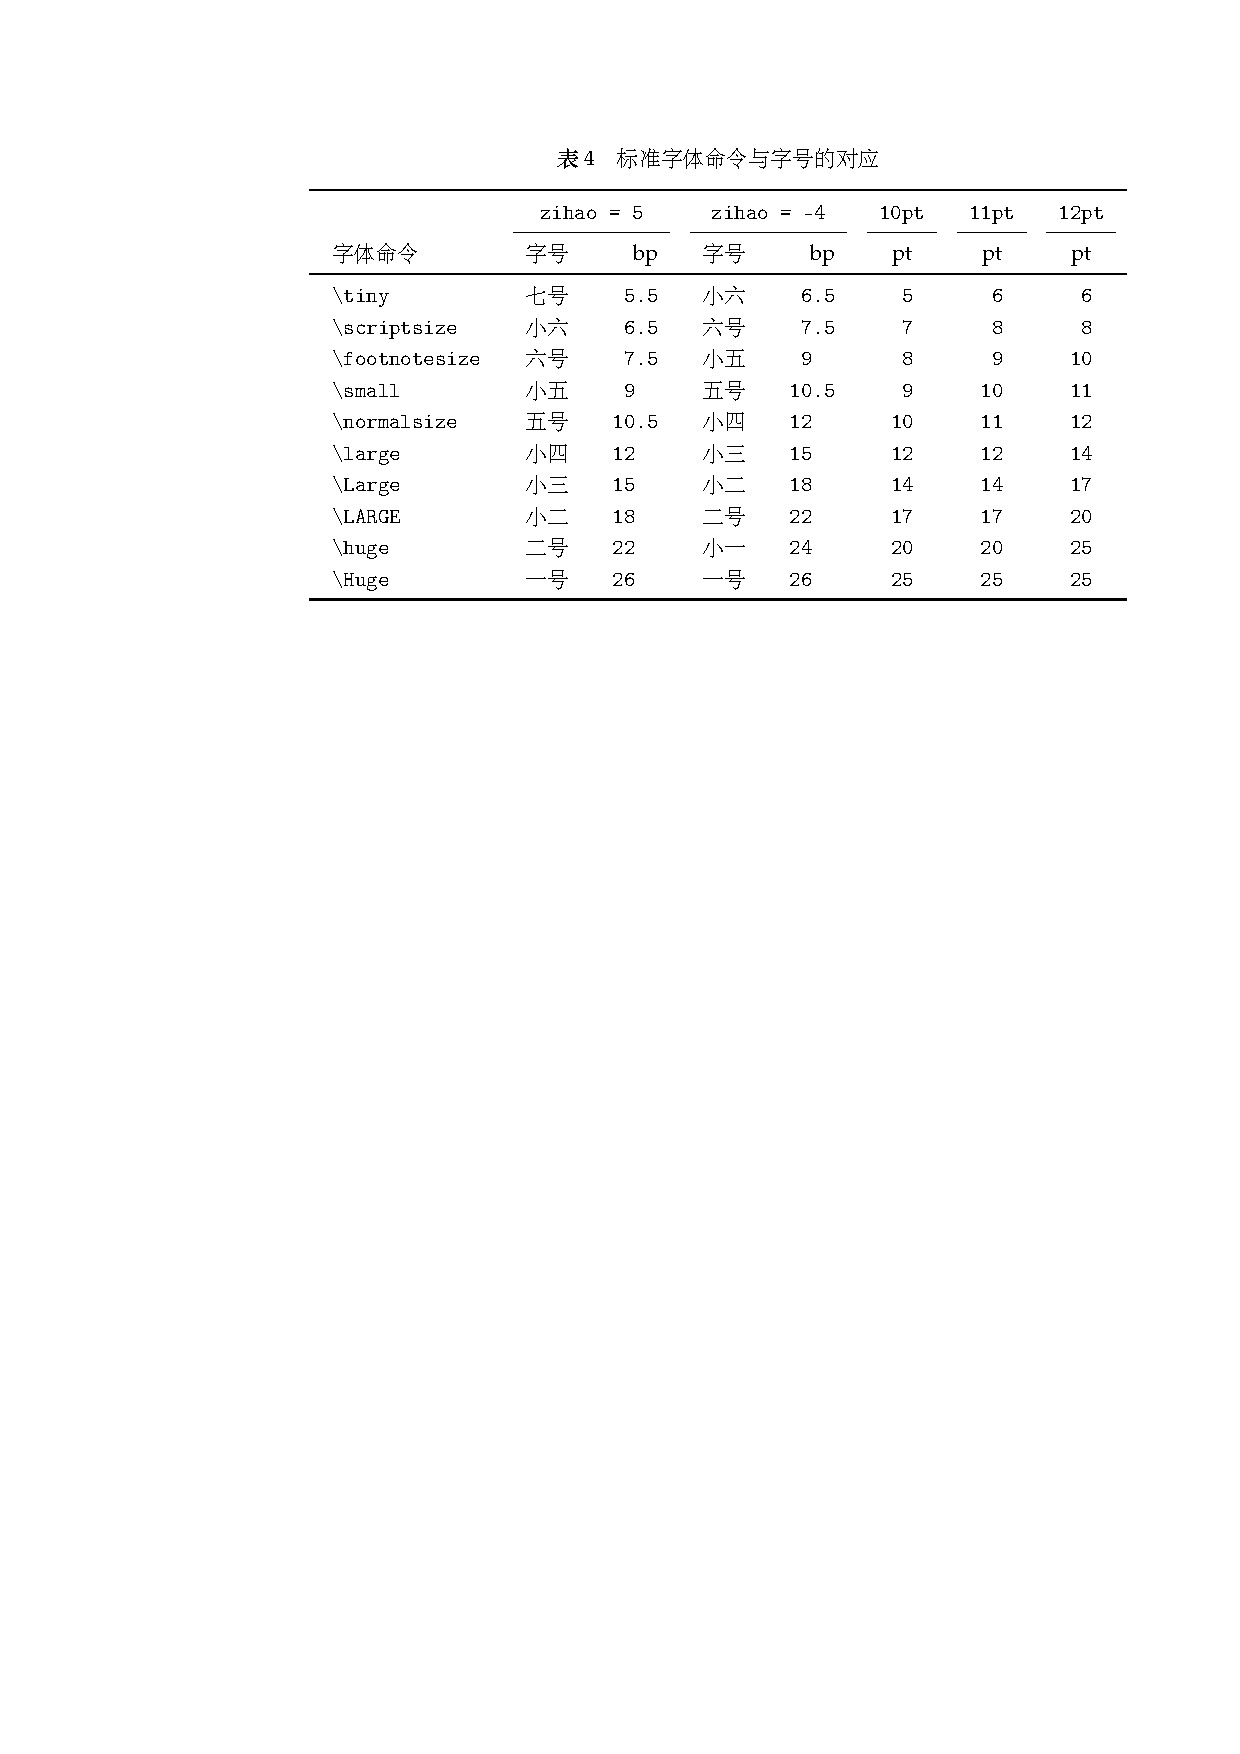
\includegraphics[scale=1]{../Pic/字号.pdf}
    \label{zihao}
\end{figure}

\subsection*{数学公式字体大小}
下面演示数学环境中相关字体大小的设置,主要会使用已经定义的命令和scalebox命令。
内置的数学公式大小主要有以下:

\bigskip
\begin{center}
    \begin{tabular}{p{22em}p{15em}}
        \toprule
        \textbf{命令} & \textbf{效果}\\
        \hline
        \cmd{displaystyle} & \ensuremath{\displaystyle \int_{x=1}^{+\infty}{\sin(x) dx}} \\
        ~\\
        \cmd{textlaystyle} & \ensuremath{\textstyle \int_{x=1}^{+\infty}{\sin(x) dx}} \\
        ~\\
        \cmd{scriptstyle} & \ensuremath{\scriptstyle \int_{x=1}^{+\infty}{\sin(x) dx}} \\
        ~\\
        \cmd{scriptscriptstyle} & \ensuremath{\scriptscriptstyle \int_{x=1}^{+\infty}{\sin(x) dx}} \\
        ~\\
        \hline\\
        \textbf{使用scalebox命令(效果不好,不推荐)}\\
        \verb |\scale{2}{<displaystyle Formular>}| & \scale{2}{\ensuremath{\displaystyle \int_{x=1}^{+\infty}{\sin(x) dx}}}\\
        ~\\
        \verb |\scale{2}{<textstyle Formular>}| & \scale{2}{\ensuremath{\textstyle \int_{x=1}^{+\infty}{\sin(x) dx}}}\\
        \bottomrule
    \end{tabular} 
\end{center}

\section{\LaTeX 数学公式的背后}

在  \TeX 程序中, 数学符号被归纳为7个基本的类别
\begin{framed}
\begin{enumerate}
    \item \textbf{普通符号[Ord]}: 拉丁字母(a),数字(1), 希腊字母($\alpha$)等
    \item \textbf{巨算符[Op]}: 求和符号($\displaystyle\sum$),积分号($\displaystyle\int$),求积符号($\displaystyle\prod$)
    \item \textbf{二元运算符号[Bin]}: 加号($+$),乘号($\times$),并集($\cup$),加减($\pm$)等
    \item \textbf{左括号[Open]}: \ensuremath{\bm {(~~~~~ [~~~~~ \{~~~~~ <}}
    \item \textbf{右括号[Close]}: \ensuremath{\bm {)~~~~~ ]~~~~~ \}~~~~~ >}}
    \item \textbf{标点符号[Punct]}: \ensuremath{\bm{;~~~~~,~~~~~.}}  
\end{enumerate}
\end{framed}

同时在数学公式中还有基线(\textbf{Baseline})和数学轴(\textbf{MathAxis})的概念。这其中各个类别的数学符号放置的
规律如下:
\begin{framed}
    \begin{enumerate}
        \item 分数线沿轴放置
        \item 括号,运算符等相对于轴(\textbf{MathAxis})对称放置
        \item 正文和上下标之比为: \textbf{10:7:5}
        \item 上下标的位置:\textbf{最简单}的情况下就是相对于基线移动一定距离
    \end{enumerate}
\end{framed}




% \subsection{数学公式中的括号大小问题}
% \begin{align*}
%     \lgroup
%         1\\2\\3\\4\\5\\6\\7\\8
%     \rgroup
% \end{align*}


\end{document}